% =============================================================================
% Draft mục 3.3.1 — Smart Contract Layer (HTLC)
% Đặt trong c3/ và \input{} vào c3_chapter.tex sau khi rà soát.
% =============================================================================

\subsection{Smart Contract Layer (HTLC)}
\label{sec:smart-contract-layer}

Lớp smart contract là tầng cao nhất quyết định việc chuyển giao tài sản
giữa các chuỗi. Trong OceanLink, lớp này gồm ba phiên bản giống nhau của
hợp đồng \texttt{HashedTimelockERC20} được triển khai trên Ethereum, Arbitrum và Base. Hợp đồng cài đặt một biến
thể \emph{multi-fill} của giao thức Hashed Time-Locked Contract (HTLC)
nhằm hỗ trợ thanh toán nguyên tử (atomic settlement) cho cả các vòng
khớp lệnh nhiều bên do Matching Engine tạo ra.

\subsubsection*{Thuật toán HTLC}

HTLC là một thuật toán mật mã đã được phát triển từ lâu nhưng chưa được thương mại
hoá rộng rãi, nó được biết đến chủ yếu trong giới nghiên cứu và một
số giao thức thanh toán xuyên chuỗi điển hình như Lightning Network
và các giao thức atomic swap giữa Bitcoin và Ethereum, song vẫn chưa
hiện diện trong các sản phẩm bridge thương mại phổ biến hiện nay.
Mô hình cơ bản giữa hai bên $A$ và $B$ trên hai chuỗi khác nhau như
sau:

\begin{enumerate}
  \item Người gửi $A$ chọn một bí mật ngẫu nhiên $s$ và tính
    $h = \mathcal{H}(s)$, với $\mathcal{H}$ là hàm băm an toàn.
  \item \emph{Pha 1 — khởi tạo HTLC trên chuỗi nguồn.} $A$ gọi hợp
    đồng trên chuỗi 1, khoá tài sản với hashlock $h$ và timelock
    $T_A$; thông tin giao dịch được chuyển sang $B$ qua kênh
    off-chain.
  \item \emph{Pha 2 — khởi tạo HTLC đối ứng trên chuỗi đích.} Sau
    khi quan sát được HTLC bên chuỗi 1, $B$ tạo một HTLC tương ứng
    trên chuỗi 2 với cùng hashlock $h$ và timelock $T_B < T_A$ (để
    $B$ luôn còn đủ thời gian xử lý nếu $A$ rút trễ).
  \item \emph{Pha 3 — $A$ rút tài sản trên chuỗi đích.} $A$ cung cấp
    preimage $s$ cho hợp đồng trên chuỗi 2 và nhận tài sản; thao tác
    này \emph{tiết lộ $s$ trên chuỗi}.
  \item \emph{Pha 4 — $B$ rút tài sản trên chuỗi nguồn.} Khi $s$ đã
    công khai, $B$ đọc nó từ event của chuỗi 2 và dùng để rút tài sản
    đã bị $A$ khoá ở Pha 1. Nếu một trong hai bên không hoàn tất
    trước timelock tương ứng, hợp đồng cho phép \emph{refund} tự
    động.
\end{enumerate}

Điểm cốt lõi là \emph{cùng một preimage $s$ mở khoá được nhiều HTLC
khác chuỗi}, nhờ đó mọi nhánh thanh toán hoặc cùng diễn ra hoặc cùng
được hoàn lại — tính nguyên tử (atomicity) được duy trì mà không cần
tin cậy bên thứ ba. Hình \ref{fig:htlc-sequence} minh hoạ bốn pha
trên dưới dạng sequence diagram giữa hai người dùng $A$, $B$ và hai
hợp đồng smart contract trên hai chuỗi.

\begin{figure}[H]
  \centering
  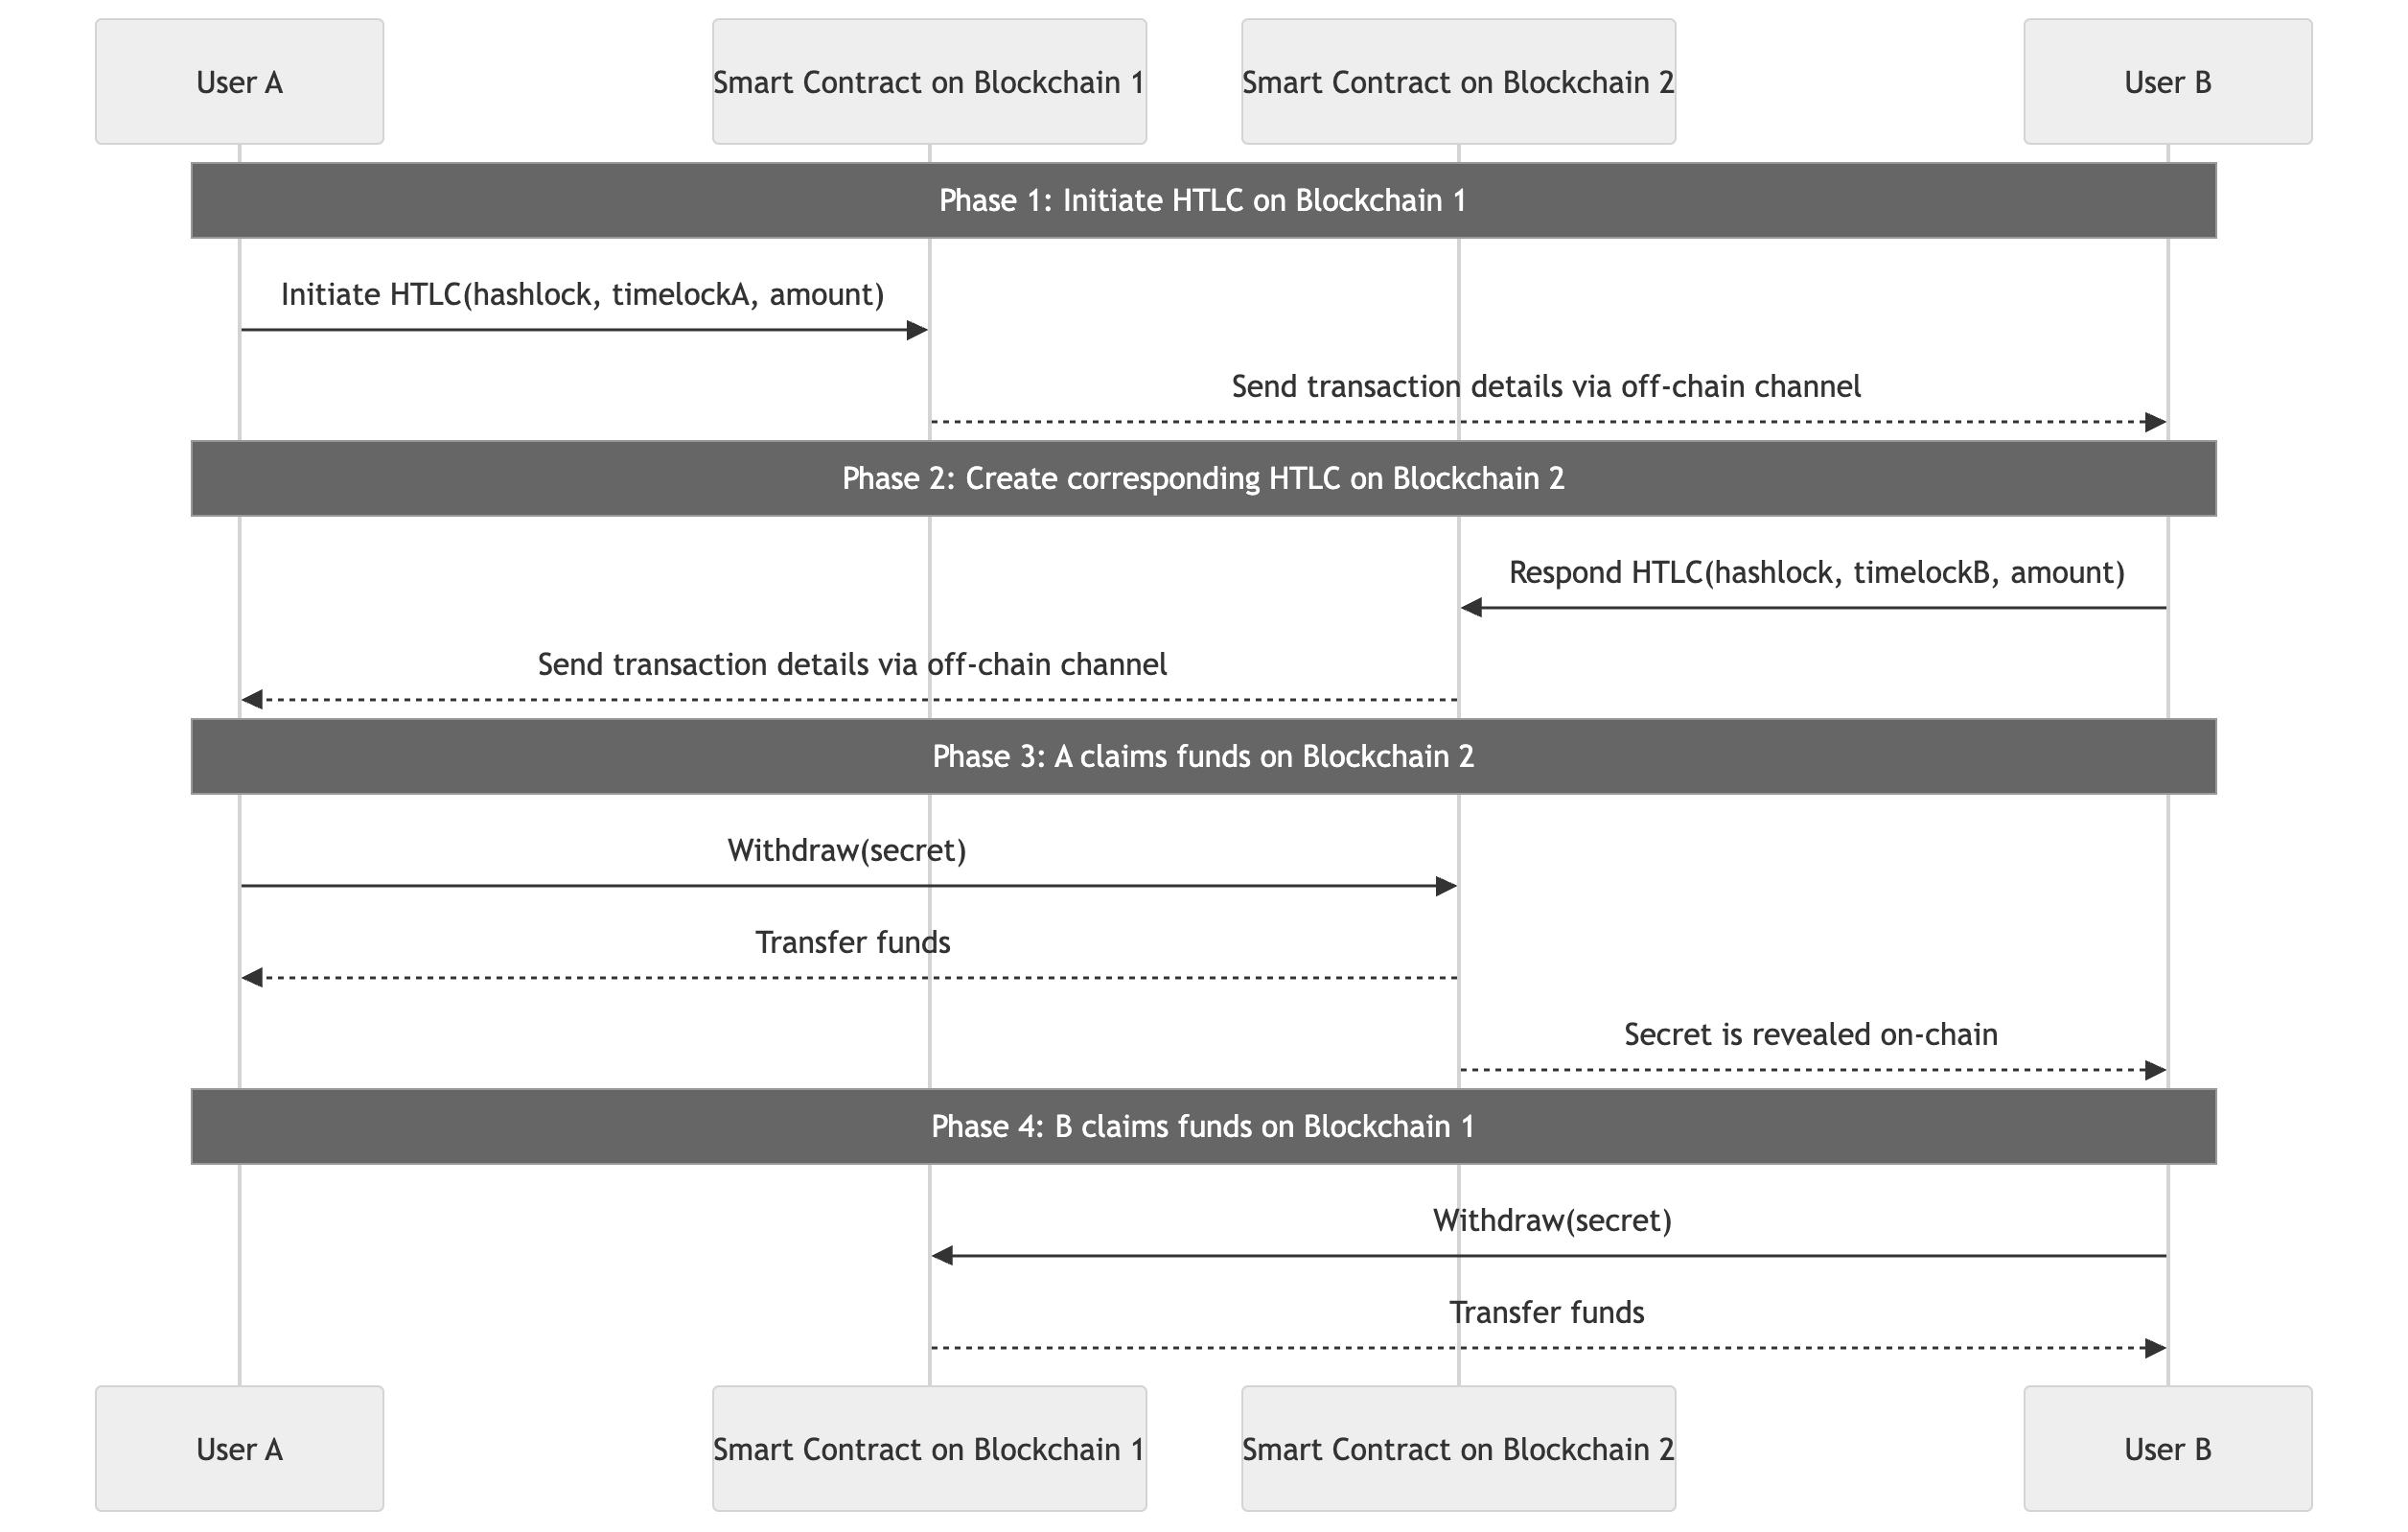
\includegraphics[width=\linewidth]{figures/c3/htlc-sequence}
  \caption{Biểu đồ tuần tự thuật toán HTLC giữa hai bên trên hai
  chuỗi}
\end{figure}

\subsubsection*{Multi-fill HTLC: thiết kế trong OceanLink}

HTLC chuẩn giả định mỗi hợp đồng tương ứng với \emph{một} cặp gửi–nhận.
Với matching theo vòng (cycle netting), trên cùng một chuỗi nguồn có
thể có nhiều người nhận khác nhau cần được thanh toán cùng một lúc, mỗi
người ứng với một hashlock riêng. Để giảm chi phí gas và đơn giản hoá
việc điều phối, OceanLink mở rộng HTLC theo hướng đa nhánh: mỗi
\textbf{Order} (đơn) chứa một hoặc nhiều \textbf{Fill} (nhánh thanh
toán). Cấu trúc dữ liệu chính được tóm tắt như sau:

\begin{itemize}
  \item \textbf{Order}: đại diện cho khoản tiền được \emph{một}
    người gửi khoá vào hợp đồng. Bao gồm: địa chỉ người gửi, token, tổng
    số tiền đã nạp, số tiền còn lại chưa được rút, thời gian khoá
    (\texttt{timelock}), trạng thái (\texttt{OPEN}/\texttt{REFUNDED}) và
    số lượng nhánh (\texttt{fillCount}).
  \item \textbf{Fill}: đại diện cho \emph{một} nhánh thanh toán bên
    trong order. Bao gồm: địa chỉ người nhận, số tiền của nhánh, hashlock
    và cờ \texttt{claimed}.
\end{itemize}

Một cấu trúc Order – Fill cho phép một giao dịch khoá tiền duy nhất phục
vụ nhiều cặp gửi–nhận, mỗi cặp được mở khoá độc lập bằng preimage tương
ứng.

\subsubsection*{Ba thao tác chính}

Hợp đồng cung cấp ba thao tác bên ngoài, tương ứng với ba pha của vòng
đời một order:

\paragraph{(1) \texttt{newOrder}.} Tạo order và đồng thời tạo toàn bộ
fill bên trong nó. Tham số gồm token, tổng số tiền, timelock và ba
mảng song song \texttt{receivers}, \texttt{amounts}, \texttt{hashlocks}.
Hợp đồng kiểm tra:

\begin{itemize}
  \item Token khác địa chỉ không, tổng số tiền dương, timelock thuộc
    tương lai.
  \item Ba mảng có cùng độ dài và không rỗng.
  \item Mỗi receiver khác địa chỉ không, mỗi amount dương.
  \item Tổng \texttt{amounts} không vượt quá số token thực sự nhận
    được sau khi gọi \texttt{transferFrom} (tính cả token có cơ chế
    \emph{fee-on-transfer}).
\end{itemize}

Sau khi xác thực, hợp đồng tăng định danh \texttt{nextOrderId}, ghi lại
order, sinh các fill và phát các sự kiện \texttt{OrderCreated} cùng
\texttt{FillCreated}. Phần token dư (\emph{dust}) — nếu tổng các fill
nhỏ hơn lượng thực sự nhận — được trả lại cho người gửi.

OceanLink cho phép một địa chỉ \emph{admin} đã được whitelist tạo order
\emph{thay mặt} một người dùng khác qua tham số \texttt{onBehalfOf}.
Tính năng này được Orchestrator sử dụng để gom nhiều fill cùng chuỗi
vào một giao dịch duy nhất, giúp tiết kiệm gas.
Khi \texttt{onBehalfOf} khác \texttt{msg.sender}, hợp đồng yêu cầu
\texttt{msg.sender} thuộc danh sách admin và token được kéo từ địa chỉ
\texttt{onBehalfOf}.

\paragraph{(2) \texttt{withdraw}.} Người nhận của một fill cụ thể (hoặc
một admin) cung cấp preimage để rút phần tiền của mình. Hợp đồng kiểm
tra:

\begin{itemize}
  \item Order tồn tại, đang ở trạng thái \texttt{OPEN}.
  \item Trừ khi cờ bất biến \texttt{allowWithdrawAfterExpiry} được bật
    lúc deploy, không cho rút sau \texttt{timelock}.
  \item Fill chưa từng được claim trước đó.
  \item $\mathcal{H}(\text{preimage}) = \text{hashlock}$, với
    $\mathcal{H}$ là hàm \texttt{sha256} của Solidity.
\end{itemize}

Theo nguyên tắc Checks–Effects–Interactions, hợp đồng đặt
\texttt{fill.claimed = true} và giảm \texttt{order.remainingAmount}
\emph{trước} khi gọi \texttt{safeTransfer} chuyển token cho người nhận.
Modifier \texttt{nonReentrant} cộng với mẫu CEI loại bỏ rủi ro tấn công
re-entrancy.

\paragraph{(3) \texttt{refund}.} Sau khi \texttt{timelock} hết hạn,
người gửi (hoặc admin) có thể gọi \texttt{refund} để lấy lại toàn bộ
phần tiền chưa được claim. Hợp đồng cập nhật trạng thái sang
\texttt{REFUNDED} và đặt \texttt{remainingAmount} về 0 trước khi chuyển
token. Đây là \emph{liveness escape hatch}: nếu vì bất kỳ lý do gì
preimage không được công bố trong thời gian khoá, tài sản không bị
khoá vĩnh viễn.

\subsubsection*{Thanh toán nguyên tử cho một vòng nhiều bên}

Để minh hoạ cách multi-fill HTLC bảo đảm tính nguyên tử cho một vòng
khớp lệnh nhiều bên, xét vòng có ba bên $A \to B \to C \to A$, mỗi
bên gửi USDC trên chuỗi nguồn của mình tới bên kế tiếp:

\begin{enumerate}
  \item Orchestrator gom các nhánh cùng chuỗi vào các \emph{order
    consolidated}. Một order trong số đó được chỉ định là \emph{order
    chủ tịch} (presiding); những order còn lại là \emph{order phản hồi}
    (responding).
  \item Order chủ tịch sinh tươi các bí mật $s_i$ và publish các
    hashlock $h_i = \mathcal{H}(s_i)$ qua sự kiện \texttt{FillCreated}.
  \item Các order phản hồi \emph{tái sử dụng} các hashlock $h_i$ này
    khi tạo HTLC trên các chuỗi khác. Như vậy mọi nhánh thuộc cùng
    một cặp đối ứng đều bị khoá bởi cùng một bí mật.
  \item Sau khi tất cả các HTLC đã có mặt trên chuỗi, Orchestrator gọi
    \texttt{withdraw} với các preimage tương ứng. Vì các preimage
    được công khai trên chuỗi qua sự kiện
    \texttt{FillWithdrawn}, mọi bên nhận ở mọi chuỗi đều có thể quan
    sát và sử dụng để rút phần của mình.
  \item Nếu bước nào đó thất bại, các HTLC chưa được rút sẽ tự động
    được hoàn lại sau \texttt{timelock}; không có nhánh nào bị mất
    vĩnh viễn.
\end{enumerate}

Tính chất an toàn cốt lõi của thiết kế: \emph{biết một preimage
$s_i$ là điều kiện đủ để mở khoá tất cả các nhánh chia sẻ
$h_i$ trên mọi chuỗi}. Cộng với cơ chế refund-after-timelock, hệ
thống thoả tính chất \textbf{liveness} (tài sản luôn về tay đúng
chủ hoặc trở về người gửi) và \textbf{safety} (không có trạng thái mà
một bên mất tài sản trong khi bên đối ứng vẫn được nhận).

\subsubsection*{Một số cân nhắc kỹ thuật}

\begin{itemize}
  \item \textbf{Hàm băm.} Sử dụng \texttt{sha256} thay vì
    \texttt{keccak256} để dễ đồng bộ với các nguyên thủy của các
    blockchain non-EVM trong tương lai (Bitcoin, Cosmos), nơi
    \texttt{sha256} là tiêu chuẩn de facto.
  \item \textbf{Bảo vệ re-entrancy.} Mọi hàm thay đổi trạng thái
    đều được khoanh bằng modifier \texttt{nonReentrant} của OpenZeppelin
    và tuân thủ mẫu CEI.
  \item \textbf{Token có fee-on-transfer.} Hợp đồng đo lượng token
    \emph{thực sự nhận được} bằng cách so sánh
    \texttt{balanceOf} trước và sau khi gọi \texttt{transferFrom},
    rồi yêu cầu tổng các fill không vượt quá số đó. Phần dư được
    trả lại người gửi.
  \item \textbf{Granularity của timelock.} Tham số
    \texttt{TIME\_LOCK} mặc định 10 phút (cấu hình qua biến môi
    trường) là sự cân bằng giữa thời gian đủ để Orchestrator hoàn
    tất nhiều giao dịch trên ba chuỗi và thời gian không quá lâu
    để khoá tài sản người dùng nếu sự cố xảy ra.
\end{itemize}
